\documentclass[12pt, a4paper]{article}
\usepackage[brazil]{babel}
\usepackage{amsmath}
\usepackage[utf8]{inputenc}
\usepackage[T1]{fontenc}
\usepackage{graphicx}
\usepackage{indentfirst}
\usepackage{hyperref}
\usepackage{url}
\urlstyle{same}
\setlength{\parindent}{1.25cm}

%Mudar orientação da página
\usepackage{lscape}

%Alterando a margem
\usepackage[margin=1in]{geometry}

%Não permitir frases estourarem a margem, principalmente urls
\sloppy

%Bibliografias
\usepackage{natbib}
\bibliographystyle{plain}

\title{Resultados do uso do algoritmo K-médias}
\author{Augusto Ribas$^1$, Bruno Nazário$^1$ e Doglas Sorgatto$^1$}
\date{$^1$Faculdade de Computação - Universidade Federal de Mato Grosso do Sul}

\begin{document}
\maketitle

\begin{abstract}
fhdfdjfdjfdjfhd
\end{abstract}
%
\section{Introdução}
jdhjdfhjdfhdhf


\subsection{Problema}
fjdhfjhfdjfd

\subsection{Objetivos}
Implementar o algoritmo K-médias sem utilizar as bibliotecas prontas disponíveis no Scikit-Learn \citep{scikit-learn} e aplicá-lo nos conjuntos de dados fornecidos pelo professor avaliando o desempenho


\section{Material e Métodos}
fhdfhdfdjfhdjfd

\subsection{Algoritmos de Agrupamento}
Clustering, ou Agrupamento,  é uma técnica de \textit{Data Mining} para fazer agrupamentos automáticos de dados segundo seu grau de semelhança. O critério de semelhança faz parte da definição do problema e, dependendo, do algoritmo conforme se lê em \citep{clustering}.

Normalmente o usuário do sistema deve escolher \textit{a priori} o número de grupos a serem detectados. Estes grupos são formados por equações que calculam a ``semelhança'' entre os dados através de funções de distância.

Os tipos de algoritmos de agrupamento de dados mais comuns são os: Particionais e os Hierárquicos. Os \emph{particionais} procuram criar grupos de semelhança.

De acordo com \citep{hierarquico}, ``Nos \emph{Hierárquico} o processo de identificação de grupos (clusters) é geralmente realimentado recursivamente, utilizando tanto objetos quanto grupos já identificados previamente como entrada para o processamento. Deste modo, constrói-se uma hierarquia de grupos de objetos, no estilo de uma árvore''.

\subsubsection{K-médias}
O algoritmo de agrupamento de dados K-Médias agrupa um conjunto de instâncias
em k partições, sendo k um número pré-estabelecido. O arranjo dos elementos é feito de maneira
que um elemento pertença a um cluster, cujo centro o elemento é mais próximo.
Dessa maneira, o algoritmo K-Médias consegue encontrar k partições disjuntas, buscando sempre
minimizar a variância intra-cluster e maximizar a variância inter-cluster. Como critérios de
convergência usuais, pode-se citar o número de iterações que o algoritmo executa e o número de
realocações de clusters.

\subsubsection{Arvore de Decisão}
fdfhdjfhdfdhj

\subsection{Procedimentos gerais}
fjdhfjdfdjfdjhf

\subsection{Conjuntos de dados}
Para este trabalho, 9 conjuntos de dados foram utilizados. Todos estes conjuntos são bi-dimensionais (isto é, têm 2 atributos), com o número de clusters variando de 2 a 10 (o primeiro conjunto tem 2 clusters, o segundo tem 3 clusters, e assim por diante). Todos estes conjuntos de dados apresentam uma partição de referência (grupo de cada um dos pontos), sendo perfeitamente balanceados (30 exemplos por grupo), como se observa na tabela \ref{conjDados}.
\begin{table}[!ht]
\centering
\caption{Características gerais dos conjuntos de dados}
\label{conjDados}
	\begin{tabular}{|l|c|c|}
	\hline
	Nome do conjunto & Número de instâncias & Número de grupos \\
	\hline
		artificial\_2.data & 60 & 2 \\
	\hline
		artificial\_3.data & 90 & 3 \\
	\hline
		artificial\_4.data & 120 & 4 \\
	\hline
		artificial\_5.data & 150 & 5 \\
	\hline
		artificial\_6.data & 180 & 6 \\
	\hline
		artificial\_7.data & 210 & 7 \\
	\hline
		artificial\_8.data & 240 & 8 \\
	\hline
		artificial\_9.data & 270 & 9 \\
	\hline
		artificial\_10.data & 300 & 10 \\
	\hline
	\end{tabular}
\end{table}

Cada um dos conjuntos de dados está disposto em um arquivo no formato CSV (\emph{``comma separated values''}). Em cada linha há um exemplo (instância) da base, no formato: $$Valor Atributo\_1, Valor Atributo\_2, Particao\_de\_Referencia$$ Sendo utilizado para o processamento apenas os dois primeiros atributos.

\section{Resultados e Discussão}

De modo geral, o algoritmo KNN obteve a maior média geral das acurácias e com maior precisão (menor variabilidade entre os resultados obtidos) como pode ser visto na tabela \ref{acuracias_geral}.


\begin{table}[!ht]
\centering
\caption{Média e desvios gerais de todas as acurácias obtidas}
\label{acuracias_geral}
\begin{tabular}{|l|l|l|}
\hline
Algoritmo & Média & Desvio Padrão\\
\hline
Árvore de decisão & 0.7549212 &0.1846360\\
Knn & 0.7872640 &0.1733436 \\
Naive Bayes &
0.7463543 &0.2417319\\
\hline
\end{tabular}
\end{table}

No entanto, dos 10 conjuntos de dados avaliados, o algorítimo Naive Bayes obteve a maior acurácia média em 7 deles, seguido do KNN que obteve a melhor acurácia em 3 e o algorítimo de Árvore de Decisão que não teve a melhor acurácia para nenhum conjunto de dados como podemos observar na tabela \ref{acuracias} e na figura \ref{acuraciasfig}

\begin{table}[!ht]
\centering
\caption{Médias obtidas por conjunto de dados para cada algoritmo}
\label{acuracias}

Média\\
\begin{tabular}{|l|l|l|l|}
\hline
Conjunto de dados & decision tree & knn & naive bayes \\
\hline                              
Banknote Authentication		&$0.9832223$ &$0.9985401$   &$0.8206231$\\
Breast Cancer               &$0.9370844$ &$0.9590793$   &$0.9634271$\\
Ecoli                       &$0.7303922$ &$0.7594474$   &$0.8104278$\\
Fertility                   &$0.8100000$ &$0.8600000$   &$0.8300000$\\
Habermans Survival          &$0.6431183$ &$0.7023656$   &$0.7453763$\\
Iris                        &$0.9266667$ &$0.9200000$   &$0.9466667$\\
Mammographic Mass           &$0.7614458$ &$0.7819277$   &$0.8096386$\\
Pima Indians Diabetes       &$0.6914046$ &$0.7460526$   &$0.7551777$\\
Planning Relax              &$0.5935673$ &$0.6210526$   &$0.6426901$\\
Yeast                       &$0.4723109$ &$0.5241747$   &$0.1395157$\\

\hline
\end{tabular}

\vspace{0.5cm}
Desvio Padrão\\
\begin{tabular}{|l|l|l|l|}
\hline                              
Conjunto de dados & decision tree & knn & naive bayes\\
\hline
Banknote Authentication    &$0.01036215$ &$ 0.003077642 $ &$ 0.06519682$\\
Breast Cancer              &$0.04473660$ &$ 0.038628010 $ &$ 0.02506400$\\
Ecoli                      &$0.16417374$ &$ 0.239384217 $ &$ 0.20628346$\\
Fertility                  &$0.12866839$ &$ 0.126491106 $ &$ 0.17029386$\\
Habermans Survival         &$0.14484407$ &$ 0.098540629 $ &$ 0.07948557$\\
Iris                       &$0.08577893$ &$ 0.075686162 $ &$ 0.06126244$\\
Mammographic Mass          &$0.04879146$ &$ 0.050305113 $ &$ 0.04536553$\\
Pima Indians Diabetes      &$0.07348156$ &$ 0.069537673 $ &$ 0.04507926$\\
Planning Relax             &$0.15234015$ &$ 0.063453212 $ &$ 0.09191607$\\
Yeast                      &$0.04864499$ &$ 0.051461378 $ &$ 0.05181031$\\

\hline
\end{tabular}

\end{table}

Para o conjunto de dados Yeast, a baixa acurácia em relação aos outros conjuntos de dados foi observada em outras tentativas também, por exemplo, Horton e Nakai \citep{horton_kenta1996} reportam uma acurácia de 55\% usando um modelo de Redes Bayesianas para classificar os exemplos enquanto Nakai e Kaneshisa \citep{nakai_kaneshisa1991} obtiveram 83\%, no entanto, para esse artigo é um precursor desse conjunto de dados, ou seja, os dados usados aqui não são exatamente os usados por estes autores, que ainda contaram com regras pre-determinadas derivadas a partir da consulta a especialistas. 

Observamos também na figura \ref{acuraciasfig} que apesar do Naive Bayes se sair bem na maioria dos casos, nos três casos onde ele obteve menor acurácia, banknote authentication, fertility e yeast, dois deles tratam de atributos em sua maioria contínuos, enquanto fertility tem somente classes hierárquicas que já são fornecidas como valores reais. No caso do "Bankbote Authentication", trata-se de atributos de imagens, parâmetros das imagens registradas de cheques legítimos e falsificados, assim imperfeições como quando se apaga palavras de um cheque original podem ser detectados. Ghazvini e colaboradores \citep{ghazvini_etal2014} também observaram uma performance inferior do Naive Bayes em relação ao algoritimo de Máquina de vetores de suporte e Redes neurais artificiais, estes autores reportam que seus melhores resultados foram obtidos com rede neural do tipo Multilayer Perceptron.

Temos também que o número de vizinhos mais próximos utilizado pelo algoritmo Knn, como observado na tabela \ref{vizinhos} é extremamente variável, sendo que para alguns conjuntos, vemos que muitos vizinhos produziam melhores resultados, enquanto outros, poucos vizinhos produziam os melhores resultados. A escolha de 11 vizinhos foi a mais comum, ocorrida para quatro conjunto de dados, mas para o conjunto de dados sobre fraudes de cheques, apenas três vizinhos deram o melhor resultado, sendo onde obtivemos a maior acurácia. Além disso, como podemos ver na figura \ref{kknn}, para conjuntos de dados como o Iris, podemos supor, que pelos resultados obtidos, que 7 é um resultado ótimo, já que ao aumentar ou diminuir o número de vizinhos para a votação da classe diminuiu a acurácia da validação cruzada, enquanto para o conjunto de dados de câncer de mama de Wisconsin (BCW), vemos que enquanto aumentávamos o número de vizinhos, ainda estávamos melhorando a acurácia, o que pode sugerir que a avaliação de valores ainda maiores do que os testados aqui podem resultar em uma maior acurácia do algoritmo, mas para manter a comparabilidade dos resultados, escolhemos a priori um conjunto de valores de vizinho mais próximos utilizados para todos os conjuntos de dados.

\begin{table}[!ht]
\centering
\caption{Número de vizinhos utilizado para o calculo de acurácia do algoritmo Knn}
\label{vizinhos}
\begin{tabular}{|l|l|}
\hline
Conjunto de dados & Número de vizinhos ótimo  \\
\hline                              
Banknote Authentication		&$3$ \\
Breast Cancer               &$11$ \\
Ecoli                       &$9$ \\
Fertility                   &$5$ \\
Habermans Survival          &$9$ \\
Iris                        &$7$ \\
Mammographic Mass           &$11$ \\
Pima Indians Diabetes       &$11$ \\
Planning Relax              &$11$ \\
Yeast                       &$9$ \\

\hline
\end{tabular}

\end{table}

Apesar da Árvore de decisão ter o pior resultado para 7 dos 10 conjuntos de dados avaliados aqui, seu resultado nunca é tão discrepante dos outros algorítimos, como quando o Naive bayes teve sua acurácia 5 vezes menor que o melhor resultado para o dados Yeast. Um ponto positivo da Árvore de decisão é a facilidade com que o seu resultado pode ser interpretado, mesmo por pessoas leigas quanto ao funcionamento do algorítimo. Ao produzir as Árvores de decisão, como apresentado na figura \ref{arvdecisao}, esse resultado pode ser facilmente interpretado e utilizado por outras pessoas \citep{berzal_etal2003}

Nossa avaliação sugere que não é simples determinar o melhor algorítimo independente do conjunto de dados. Mesmo o Naive Bayes, que teve a melhor performance geral, teve uma performance insatisfatória para alguns problemas, como por exemplo no caso de Yeast em que ele foi o pior, muito abaixo da média dos outros dois algorítimos e no caso dos Cheques falsificados, onde uma performance superior, como a obtida pelo Knn pode significar uma grande economia para os bancos. Além disso, para problemas como do Iris, onde estamos tentando classificar espécies vegetais a partir de medidas de flores, usuários finais podem ficar mais satisfeitos com uma Árvore de decisão impressa em um guia de identificação de plantas do que ter a necessidade de usar um computador para conseguir se utilizar de um modelo de classificação criado.

\begin{landscape}
\begin{figure}[!ht]
  \caption{Visão geral dos dados antes do agrupamento}
  \label{antes}
  \centering
    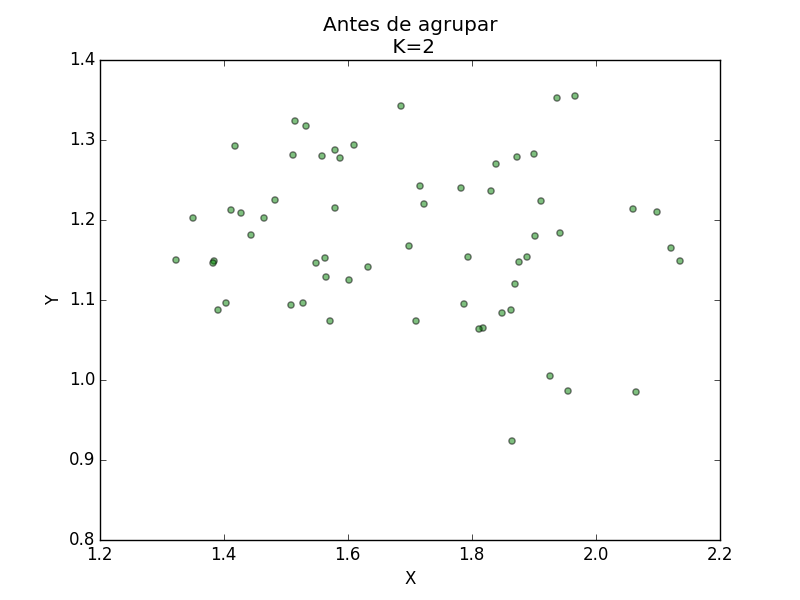
\includegraphics[width=0.4\textwidth]{antes_k2.png}
    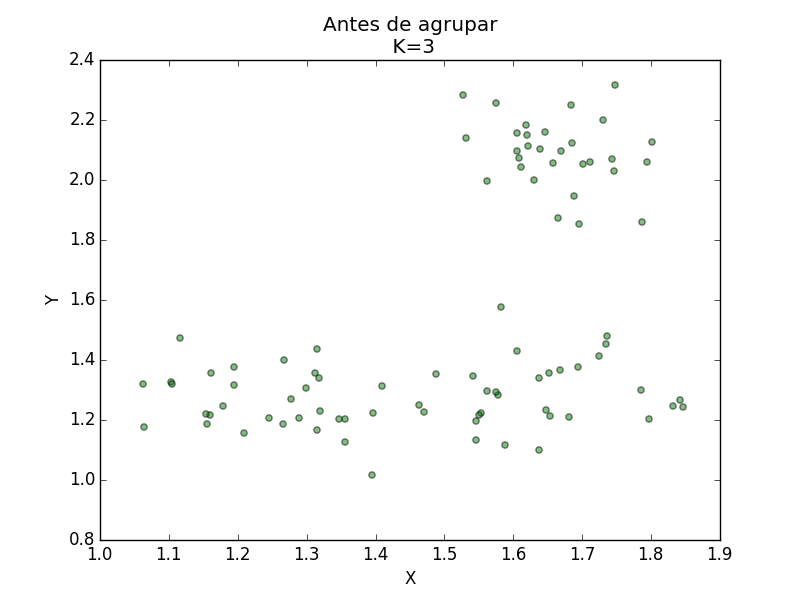
\includegraphics[width=0.4\textwidth]{antes_k3.png}
    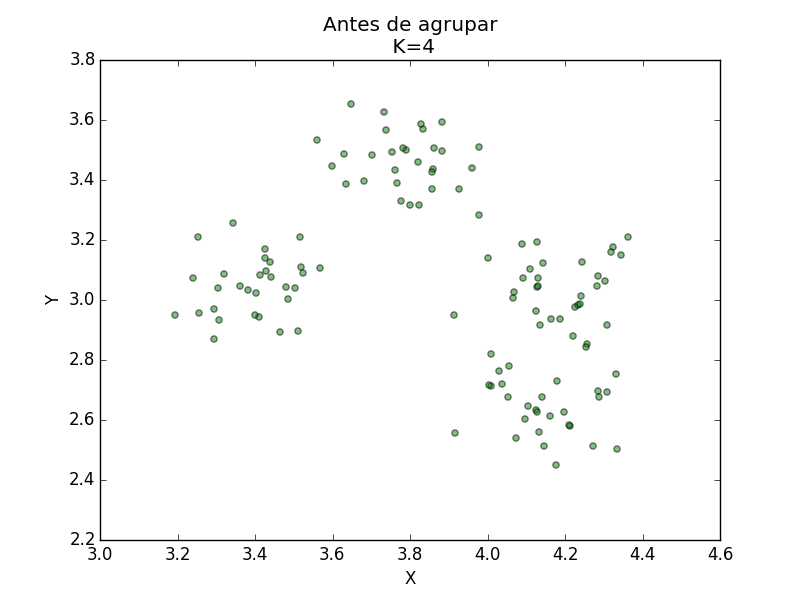
\includegraphics[width=0.4\textwidth]{antes_k4.png}
    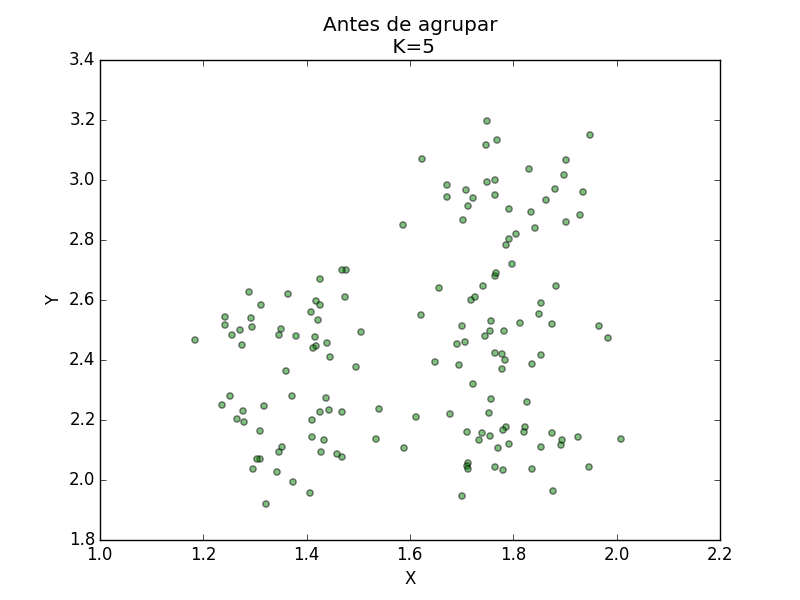
\includegraphics[width=0.4\textwidth]{antes_k5.png}
    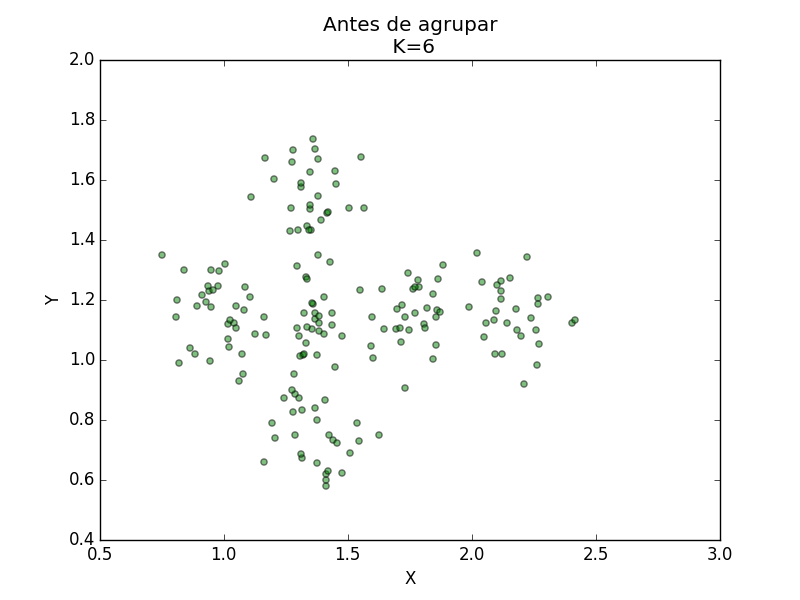
\includegraphics[width=0.4\textwidth]{antes_k6.png}
    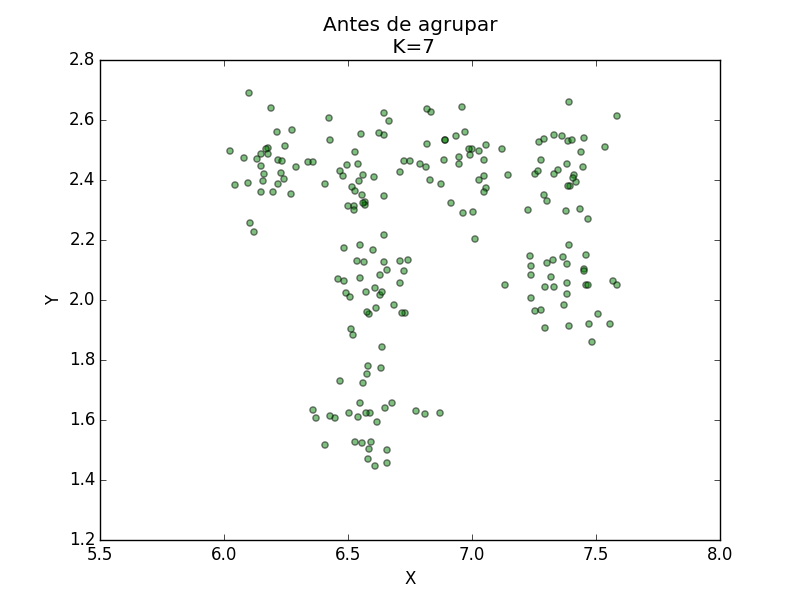
\includegraphics[width=0.4\textwidth]{antes_k7.png} 
    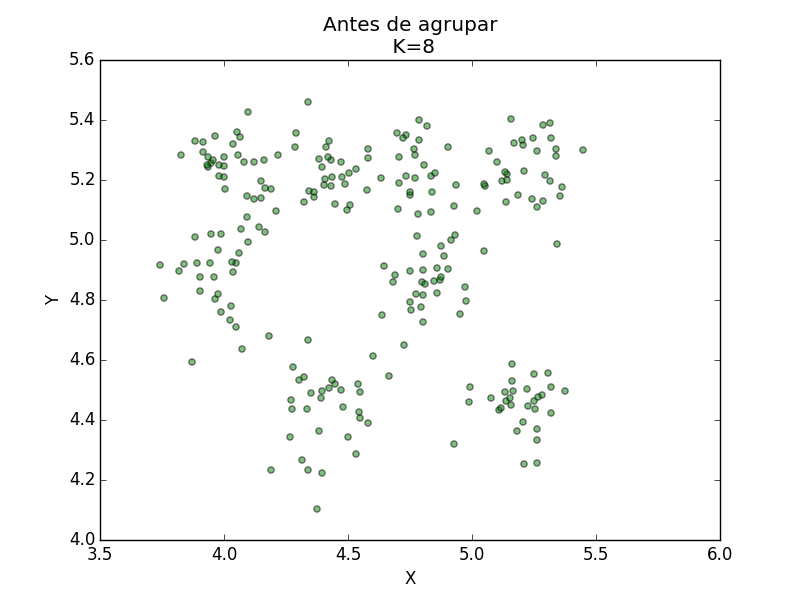
\includegraphics[width=0.4\textwidth]{antes_k8.png}    
    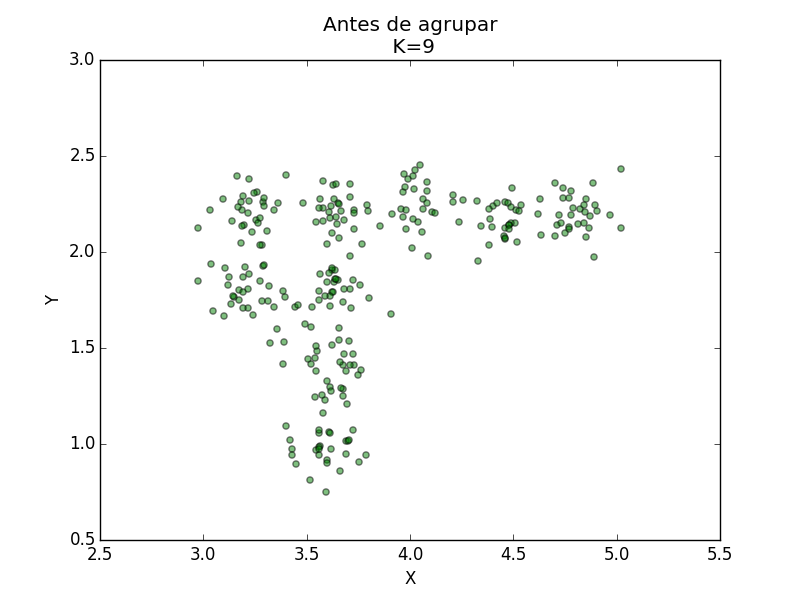
\includegraphics[width=0.4\textwidth]{antes_k9.png}
    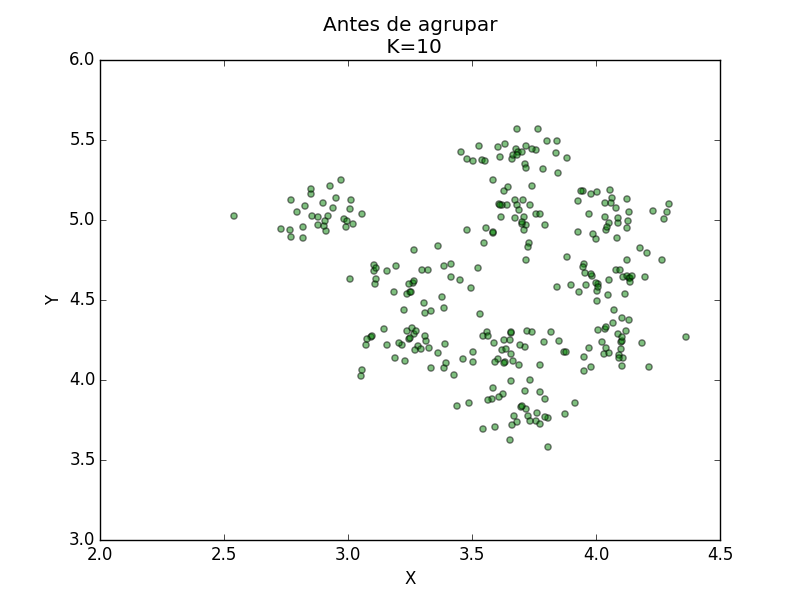
\includegraphics[width=0.4\textwidth]{antes_k10.png}          
\end{figure}
\end{landscape}

\begin{landscape}
\begin{figure}[!ht]
\label{erros}
  \caption{Evolução dos Somatórios de Erro Quadrático - SSE}
  \centering
    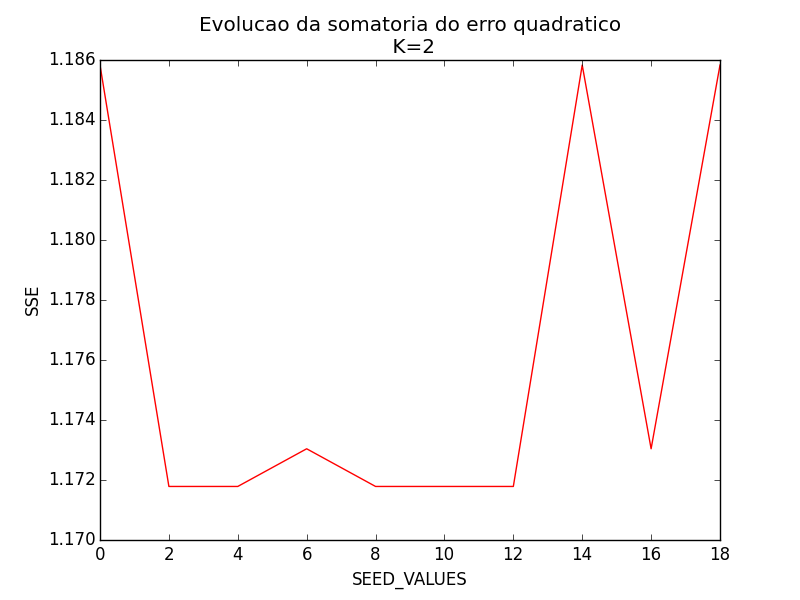
\includegraphics[width=0.4\textwidth]{erro_k2.png}
    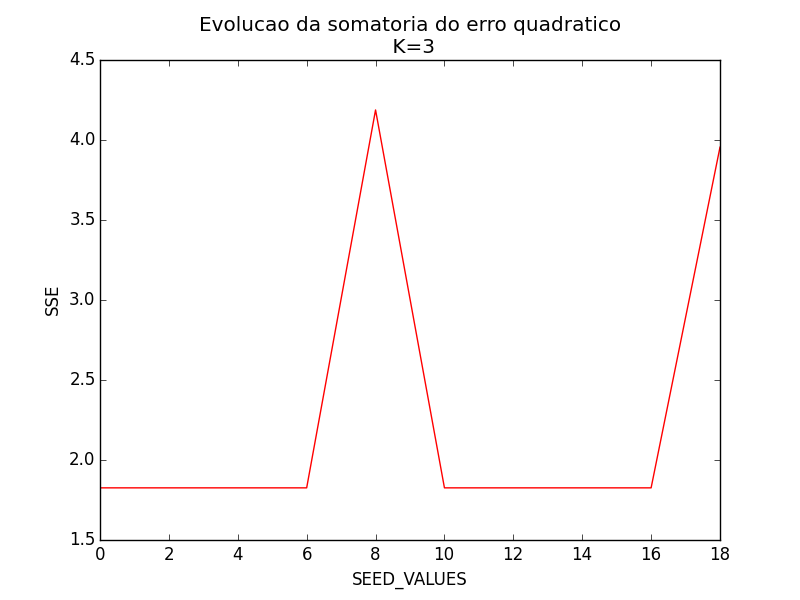
\includegraphics[width=0.4\textwidth]{erro_k3.png}
    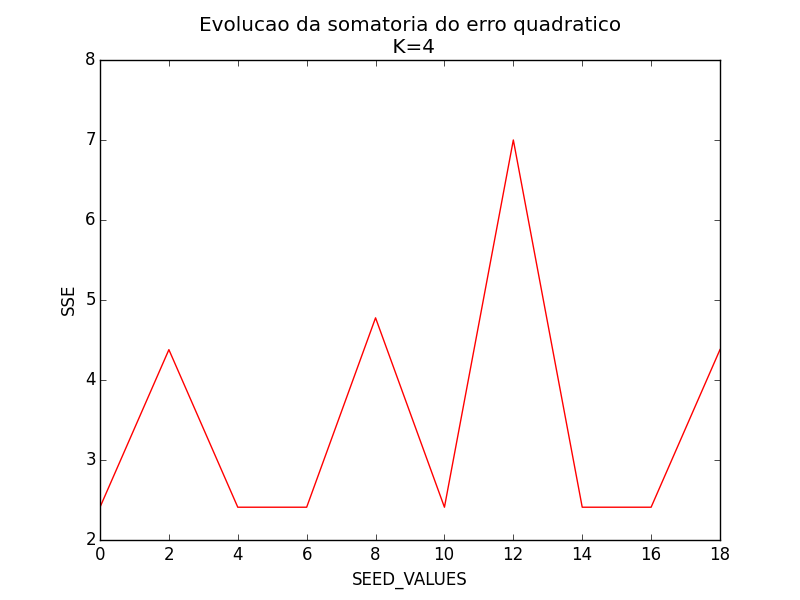
\includegraphics[width=0.4\textwidth]{erro_k4.png}
    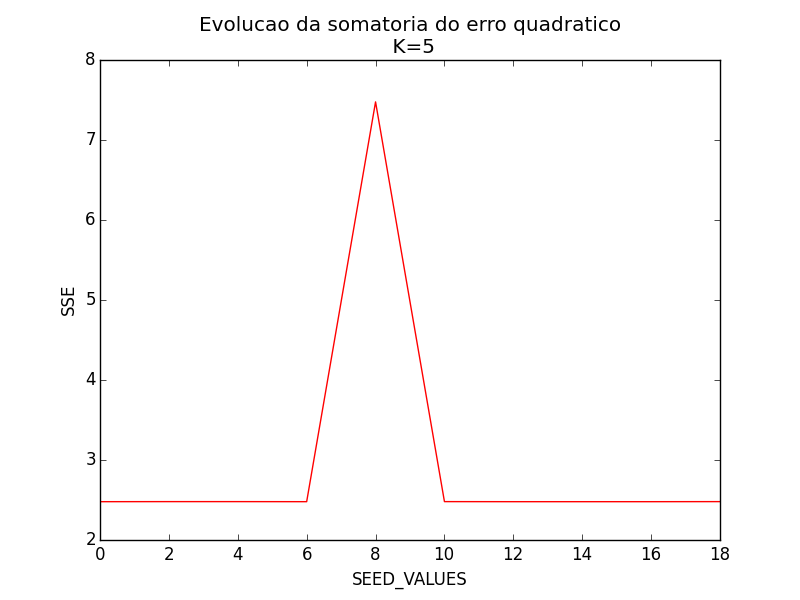
\includegraphics[width=0.4\textwidth]{erro_k5.png}
    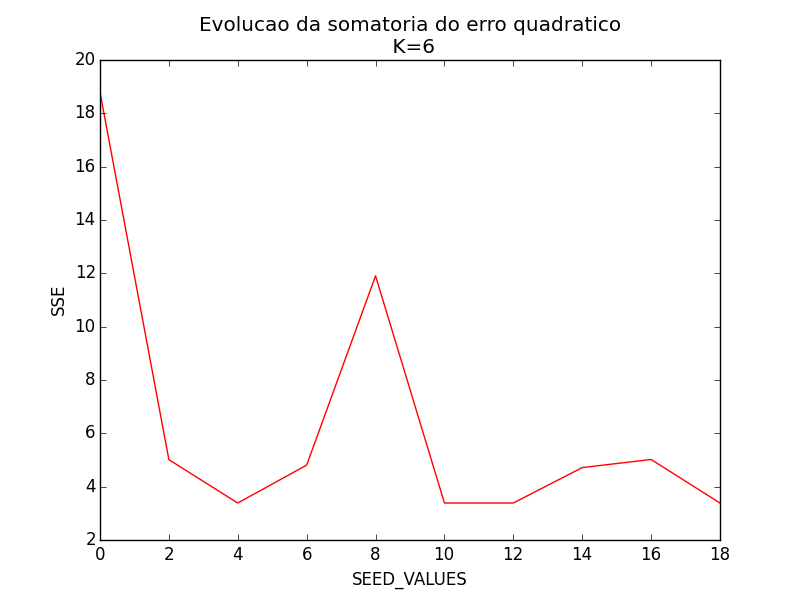
\includegraphics[width=0.4\textwidth]{erro_k6.png}
    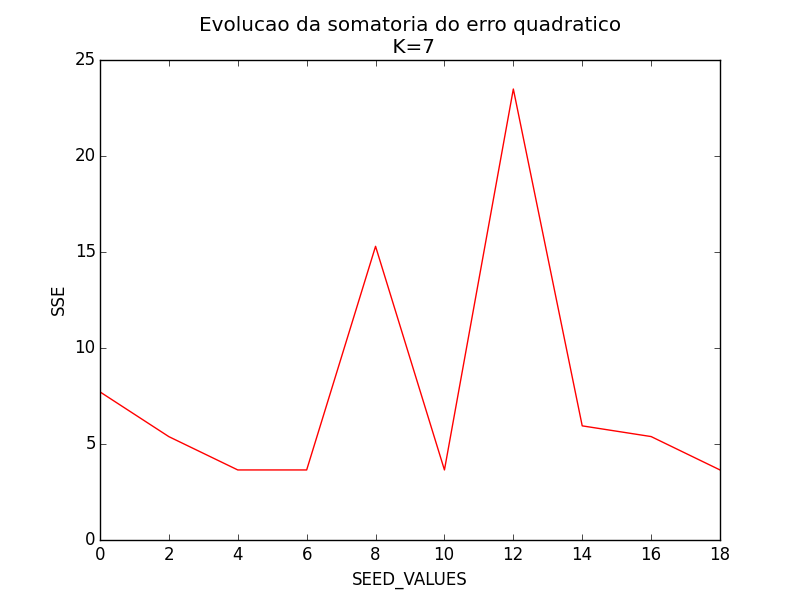
\includegraphics[width=0.4\textwidth]{erro_k7.png} 
    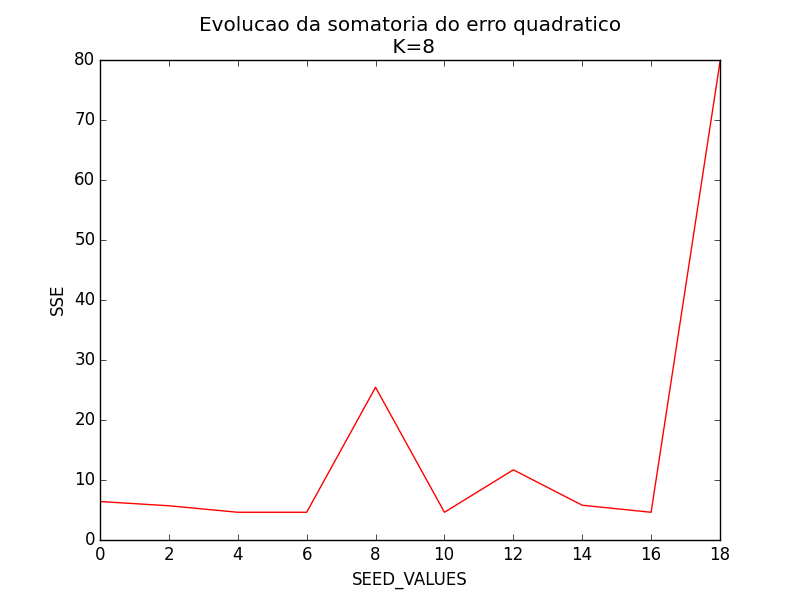
\includegraphics[width=0.4\textwidth]{erro_k8.png}    
    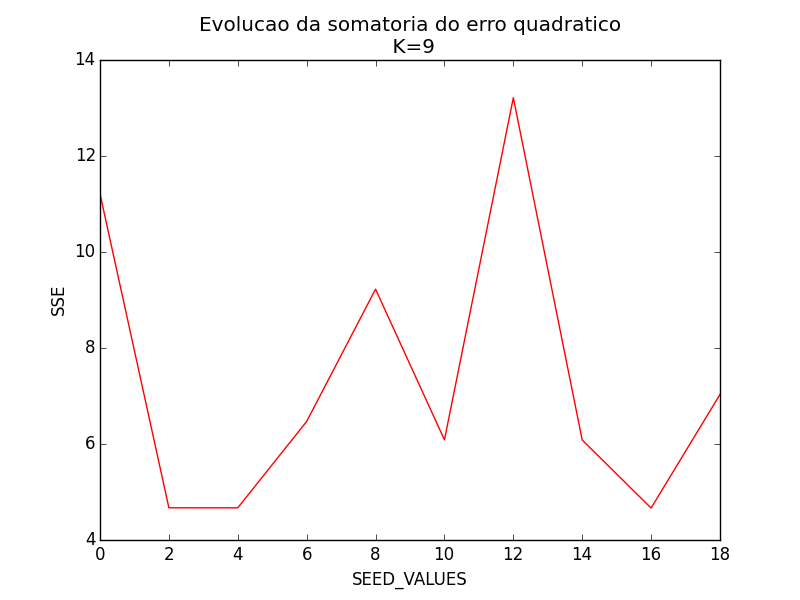
\includegraphics[width=0.4\textwidth]{erro_k9.png}
    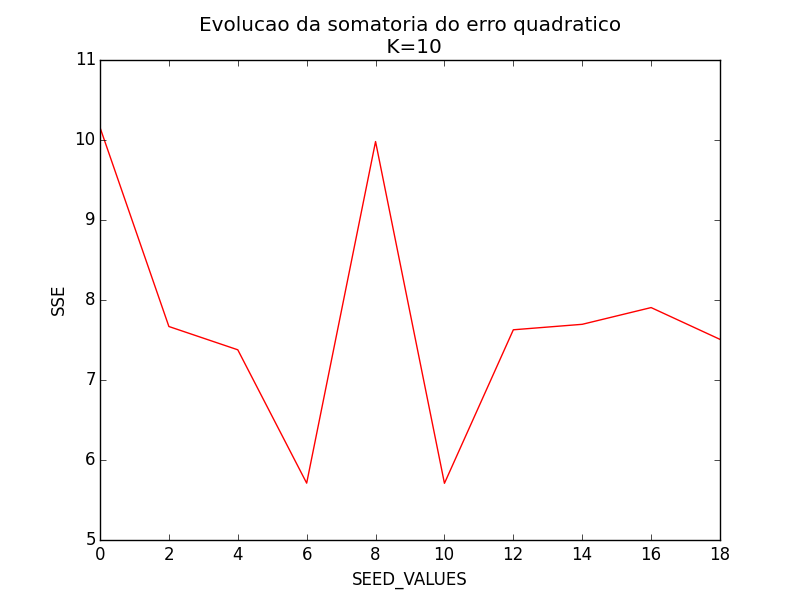
\includegraphics[width=0.4\textwidth]{erro_k10.png}
\end{figure}
\end{landscape}

\begin{landscape}
\begin{figure}[!ht]
\label{erros}
  \caption{Exemplo de evolução do processo de agrupamento para k = 5}
  \centering
    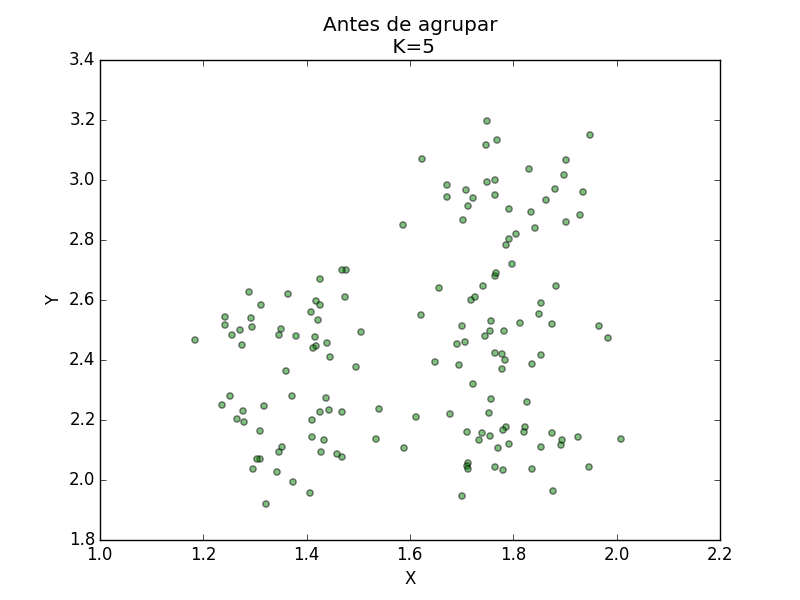
\includegraphics[width=0.4\textwidth]{antes_k5.png}
    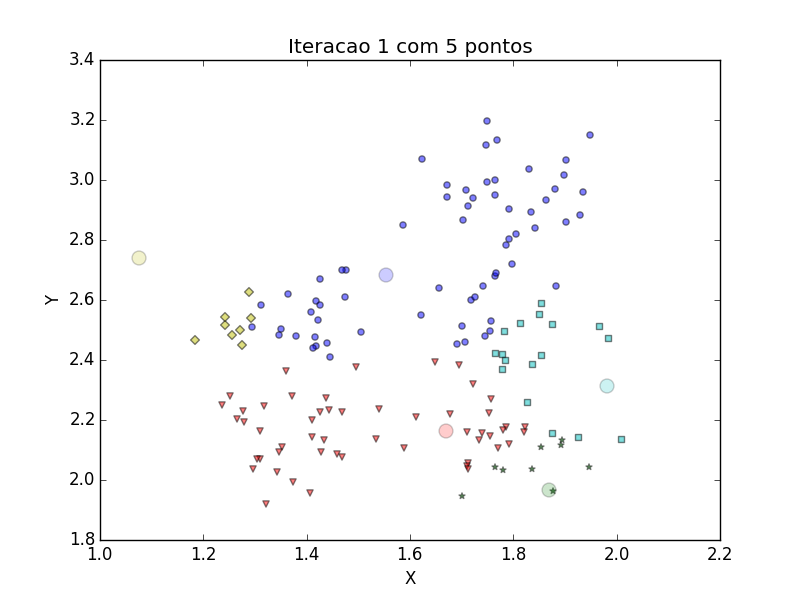
\includegraphics[width=0.4\textwidth]{depois_1.png}
    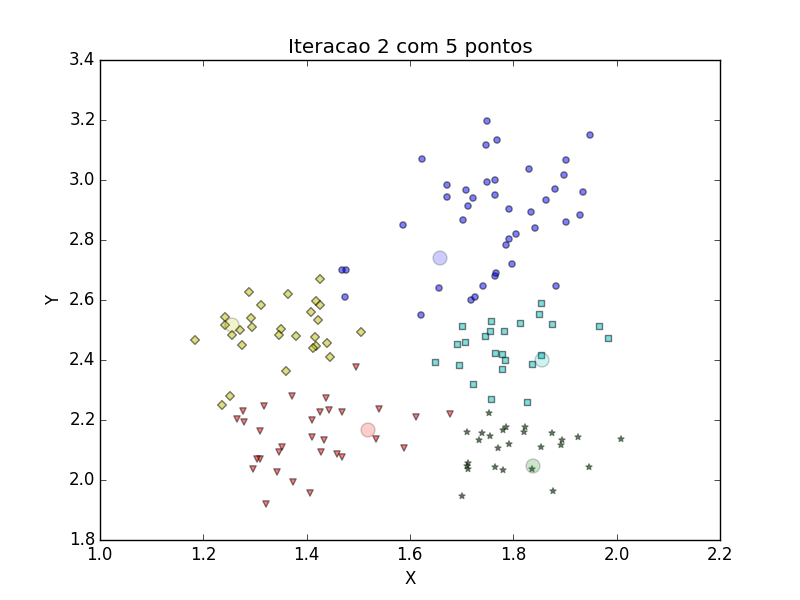
\includegraphics[width=0.4\textwidth]{depois_2.png}
    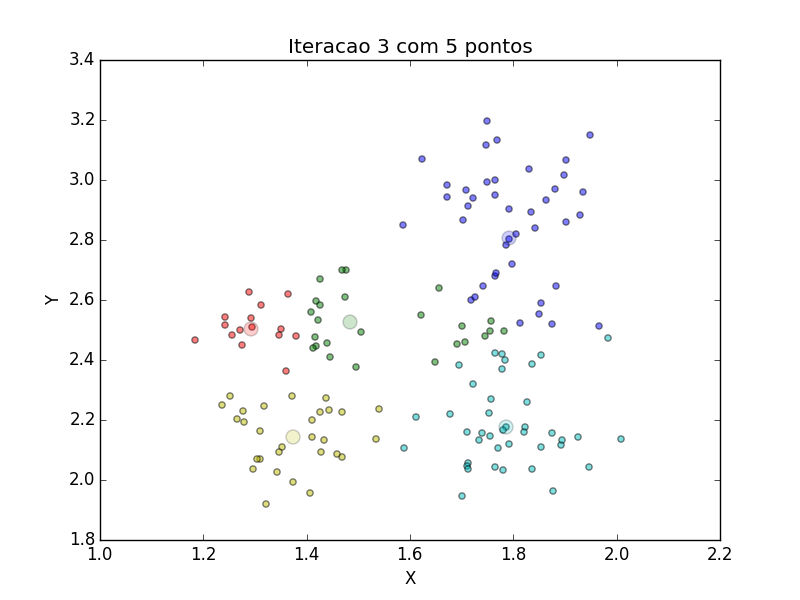
\includegraphics[width=0.4\textwidth]{depois_3.png}
    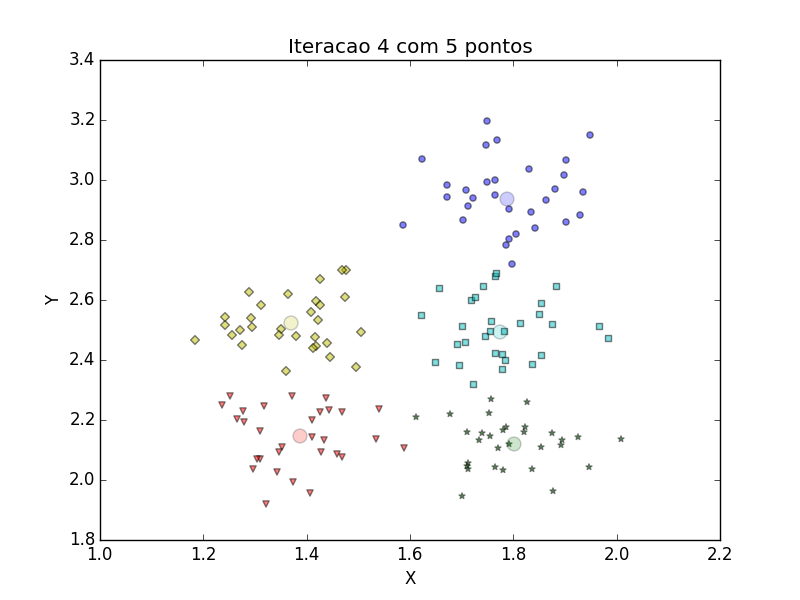
\includegraphics[width=0.4\textwidth]{depois_4.png}
    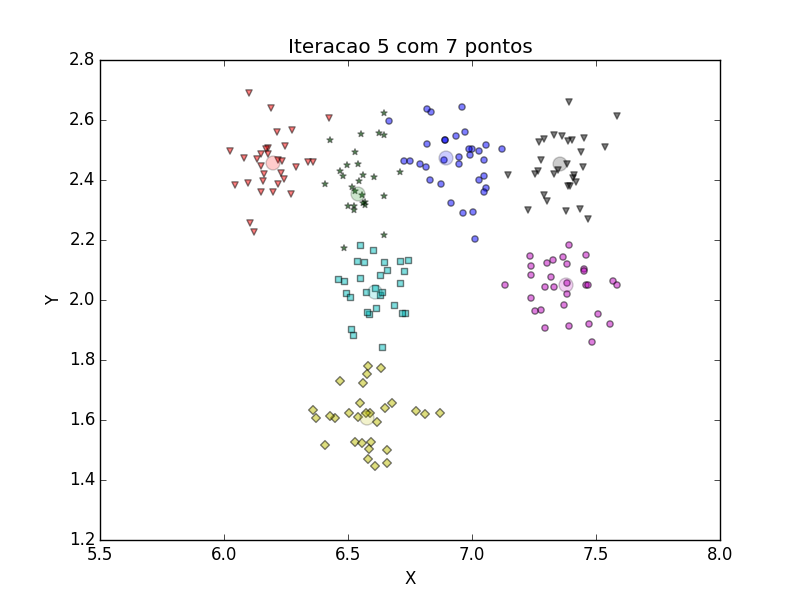
\includegraphics[width=0.4\textwidth]{depois_5.png} 
    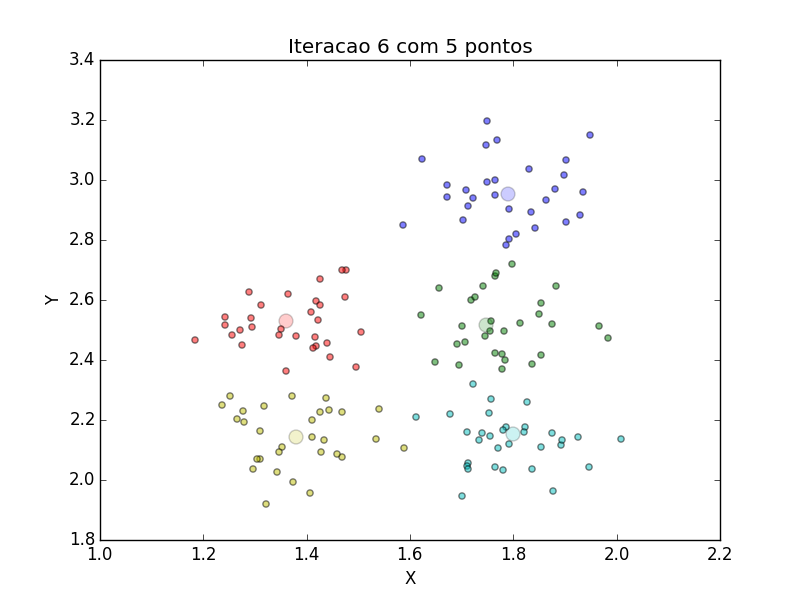
\includegraphics[width=0.4\textwidth]{depois_6.png}    
    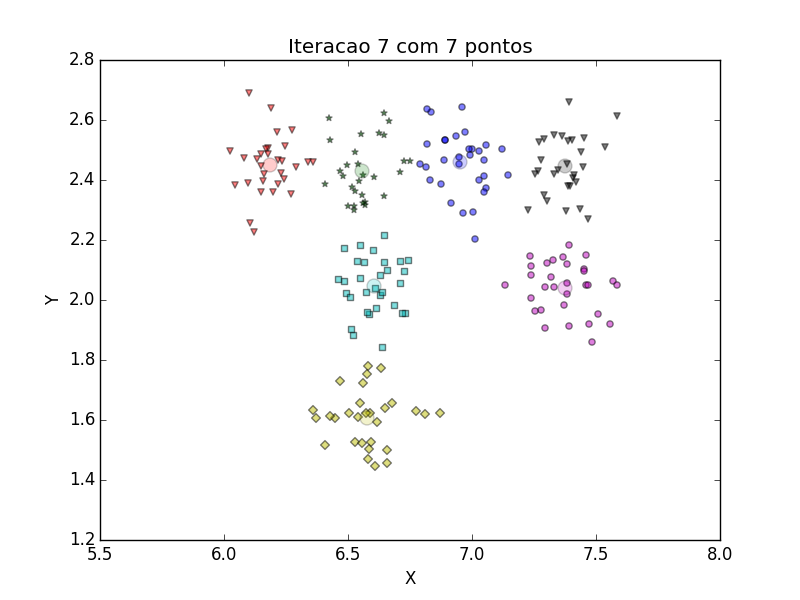
\includegraphics[width=0.4\textwidth]{depois_7.png}
    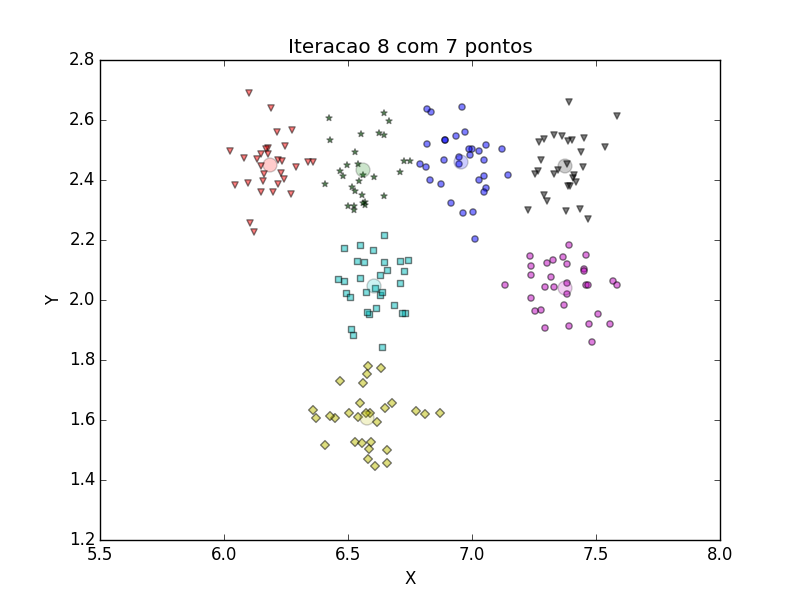
\includegraphics[width=0.4\textwidth]{depois_8.png}
\end{figure}
\end{landscape}

\newpage
\bibliography{Trabalho_IA.bib}

\end{document}